%************************************************
\chapter{Introduction to RNA design}\label{ch:review_design} % $\mathbb{ZNR}$
%************************************************
The previous chapters demonstrated the implications of \acp{ncRNA} molecules in varying levels of cellular processes, from gene expression regulation (\acp{miRNA}, \acp{piRNA}, \acp{lncRNA}) to \ac{RNA} maturation (\acp{sncRNA}, \acp{snoRNA}) and protein synthesis (\acp{rRNA}, \acp{tRNA}). Knowing that these biological functions are performed by high dimensional \ac{RNA} structures, which strongly depend on their secondary structures,  we also provided a comprehensive review of computation methods for predicting secondary structures. Now that we have computational folding tools that are accurate enough, is it possible to design an \ac{RNA} molecule that can accomplish a desired biological function for a given secondary structure? Answering this question may demand both experimental and computational efforts. For artificial \acp{ncRNA} for which the native \ac{RNA} sequence is unknown, the essential prerequisite for experimentalists is often a computational solution to the inverse folding problem. Unlike the folding situation, the inverse folding problem begins from a given secondary structure, and the goal is to find one or many  \ac{RNA} sequences that fold into that secondary structure. This chapter aims to provide the formal background and biotechnological implications of addressing this problem. Then, it gives a brief literature review of the existing computational methods. 

\section{RNA inverse folding and biotechnological implications}  
%\graffito{You might get unexpected results using math in chapter or
%section heads. Consider the \texttt{pdfspacing} option.}

In modern biotechnology, we often seek to reproduce the natural ability of the cells to control gene expressions using a variety of nucleic acids and proteins. These natural cellular abilities result from networks of regulatory molecules such as \acp{ncRNA} that dynamically regulate the expression of specific genes in response to environmental signals. Therefore, the ability to engineer biological systems is directly related to controlling gene expression. The increasing number of examples of natural regulator \acp{ncRNA} has opened doors to many emerging subfields such as \ac{RNA} synthetic biology \cite{chappell2015renaissance, isaacs2006rna} and \ac{RNA} nanostructure \cite{jaeger2001tectorna, guo2010emerging}. Researchers have engineered \ac{RNA} molecules with new biological functions, inspired by this natural versatility. Synthetic biology has also made significant progress in developing versatile and programmable genetic regulators that precisely control gene expressions in the last decades. Three general approaches are taken to engineer new functional \acp{RNA}: harvesting from nature, computational design and molecular evolution. We are interested here in computational \ac{RNA} design methods.

In most cases, designing a functional \ac{RNA} goes beyond computationally generating a set of \ac{RNA} sequences that fold into a given secondary structure. Successful design methods include computational and experimental, predictive and analytical techniques. However, computational tools addressing the inverse folding problem often provide some guidance and rationalities through the design process. For example, Steffen Mueller and his collaborators \cite{mueller2010live} suggested a systematic, rational approach, \ac{SAVE}, to develop new, productive live attenuated influenza virus vaccine candidates using computer-aided rational design. In addition, Eckart Bindewald et al. \cite{bindewald2011multistrand} used computational tools for solving inverse \ac{RNA} folding in the design of nanostructures, including pseudoknots. And in designing several \acp{ncRNA} with a successful synthetic such as ribozymes \cite{dotu2014complete}, riboswitches \cite{findeiss2015design,wachsmuth2015design}. 

Depending on the specificities of the \ac{RNA} design task, finding the underlying mathematical model that maps each designed \ac{RNA} sequence solution to a set of properties that includes most of the specifications or constraints can be a challenging task. When it exists, it allows to address the \ac{RNA} design problem computationally, and we call this mathematical model the objective function of the \ac{RNA} design problem. The complexity of the objective function used gives rise to two \ac{RNA} design problems: the negative and the positive design. The following section describes both \ac{RNA} design problems and their computational complexities.

\section{The positive and negative design}

We often find two types of \ac{RNA} design problems in the literature: negative and positive design. The negative structural design of \acp{RNA}, also called the inverse \ac{RNA} folding problem, aims to find one or many \ac{RNA} sequences that fold into a given target \ac{RNA} secondary structure while avoiding alternative folds of similar quality for the chosen energy model $\Delta G$. In other terms, it is an optimization problem where a target \ac{RNA} secondary structure $\mathcal{S}^*$ of length $L$ is given, and the goal is to determine an \ac{RNA} sequence $\phi$ of length $L$ such that $\forall \mathcal{S} \neq \mathcal{S}^* \in \Sigma_{\phi}$, $\Delta G(\phi, \mathcal{S}) > \Delta G(\phi, \mathcal{S}^*)$ .

This problem is \ac{NP}-hard even in a simple energy model \cite{bonnet2020designing}, and we cannot provide a parameterized algorithm that solves it in a polynomial time. 

In contrast, a positive design problem consists of optimizing affinity towards a given target secondary structure. In other terms, the objective is to find a sequence $\phi \in \{\text{A},\text{U},\text{C},\text{G}\}^L$ such that  $ \mathcal{S}^*=\mathcal{S}^{MFE}(\phi) = \arg \min_{\mathcal{S} \in \Sigma_{\phi}} \Delta G(\phi, \mathcal{S})$ (i.e. the sequence $\phi$ should have as \acp{MFE} structure of its ensemble $\Sigma_{\phi}$ the target structure $\mathcal{S}^*$). The positive design is computationally solvable exactly in polynomial time \cite{flamm2001design}. 

Both negative and positive designs are considered in this work, and the main difference often depends on the objective function used. In addition, it has been recently shown that the proportion of designable secondary structures decreases exponentially with $L$ for various popular combinations of energy models and design objectives \cite{yao2019exponentially}. The following section presents an overview of previously used objective functions of for the \ac{RNA} design problem.


\section{Objective functions previously used in the context of Inverse RNA folding}

%The objective function plays an essential role in any mathematical optimization problem. To address the \ac{RNA} design problem computationally, the prerequirsite is to define an appropriate objective function. Several objective functions have been previouslu used in the context of \ac{RNA} design and each of them depends on the design specifications. We provide here in this section, an overview of 

For a given target secondary structure $\mathcal{S}^*$ of length $L$, a brute force approach to the inverse \ac{RNA} folding problem that enumerates all possible \ac{RNA} sequences is not viable due to the exponential growth of the search space with increasing length (i.e. $4^L$). For the space of compatibles sequences to the target $\mathcal{S}^*$, an upper bound can be defined by restricting the paired position to the base-pairs: G-C, G-U, and A-U. This results in $6^{(L-u)/2} \times 4^u$ sequences compatible with $\mathcal{S}^*$ where $u$ is the number of unpaired nucleotides. The most common way to efficiently handle the huge set of possible solutions is to solve an optimization problem subjected to a formulated objective function. There exists a variety of well-established optimization methods helping to perform this task. However, finding the right objective function to evaluate the solutions can be quite challenging. This section of our work provides an overview of an objective function and an essential description of the most previously used objective functions in designing \ac{RNA} molecules.

The objective function defines a mathematical model that maps each \ac{RNA} sequence solution to its essential properties or functions. In biological terms, this relation between fitness and sequence can be seen as assigning a phenotype (score) to a genotype (sequence). Selection pressure due to the optimization method ensures that better phenotypes are advantageous and thus preferred, which optimizes the sequence to fall into fitness optima. This section defines the previously used objective functions in the \ac{RNA} design problems and highlights some interesting properties.
\begin{itemize}
	\item A simple distance from the target structure: in the simplest setting, the objective function of an \ac{RNA} sequence~\(\phi\) defines the distance between $\mathcal{S}^*$ and the current \ac{MFE} structure $\mathcal{S}^{MFE} (\phi)$. It often requires only the \ac{MFE} structure's computation, hence being computationally fast. There are many variants of this distance measure: base-pair distance, hamming or string edit distance, tree-edit distance and energy distance. For a formal definition of each of those distances, see \autoref{sec:rna_biochemical}. This objective function was used in the earliest tools such as \texttt{RNAinverse} \cite{hofacker1994fast} but also in many others since then \cite{andronescu2004new, busch2006info, gao2010inverse}. 
	
	\item A negative design objective function: in contrast to the above mentioned objective functions (often considered when performing a positive design), we consider the whole structural ensemble when computing the fitness of an \ac{RNA} sequence $\phi$. In most cases, it is preferable also to consider negative design goals, which allows for avoiding alternative structures of similar quality to the target structure.
	%The notion of defect often terms the avoidance of alternative structures. 
	Negative \ac{RNA} design methods usually consider one of the three following defects: (1) the \textit{suboptimal defect} \cite{hofacker1994fast, flamm2001design, dirks2003partition, zadeh2011nupack} which defines the energy distance to the first suboptimal (2) the \textit{probability defect} \cite{zadeh2011nupack, hofacker1994fast} which defines the probability that the sequence $\phi$ folds into any other structure than the target structure $\mathcal{S}^*$  and (3) the \textit{ensemble defect} \cite{zadeh2011nupack} which corresponds to the average number of incorrectly paired nucleotides at equilibrium calculated over the structure ensemble of $\phi$, $\Sigma_{\phi}$. 
	
	\item Multi-objective optimization: in some designing cases where more than one goal is specified, it is necessary to formulate an objective function for each goal. That results in a multi-objective optimization problem. The solutions to such a problem are all optimal for at least one objective function and thus arranged on the so-called Pareto optimal front. This approach has already been used in several \ac{RNA} design tools such as \texttt{Modena} \cite{modena_2012, taneda2015multi} and in \cite{ramlan2011design}.
	
	\item Bistable and multi-stable riboswitches objective functions: In some designing cases, especially for riboswitches, it is possible to specify more than one desired target structure, including the energy differences between them, the barrier heights and the kinetic properties. Following the same idea, Flamm et al. introduced an objective function that enables designing \ac{RNA} molecules to adopt two distinct structures \cite{flamm2001design}. This bistable objective function contains two terms. The first term increases the probability of both structures in the ensemble, and the second specifies the desired energy difference between both states. It is also possible to vary the states' temperature to gain a bistable thermoswitch. The same idea has therefore been expanded to an objective function for designing \ac{RNA} molecules that can adopt more than two structures, including extension for multi-structure energy barrier calculations \cite{ramlan2011design, shu2010ardesigner}.  \texttt{Frnakenstein} \cite{lyngso2012frnakenstein} also utilises such objective function for multi-target design.
	
	\item Mutational robustness and neutrality: In addition to the above-mentioned objective functions, objective functions aim to measure the mutual neutrality of the sequence concerning the target structure \cite{shu2010ardesigner}. When using such an objective function, the sequences are optimized so that the fraction of one-mutant neighbours to the original structure is as significant as possible. This allows for perfectly preserving the structure when mutations are introduced. We often talk of a mutational robustness optimization \cite{avihoo2011rnaexinv}.
\end{itemize}

These objective functions suggest that the inverse folding problem is a major challenge with no single solution yet, and many possible ways of setting the goal. This thesis relies on three objective functions: the simple distance to the target, the ensemble defect, and the mutational robustness. In addition to the many objective functions, there are also several methods. The following section will review the existing methods independently of the objective function and provide some limitations.

\section{A review on existing inverse RNA folding tools.}

Several methods or algorithms addressing this problem have been proposed in the literature. The existing techniques can be classified into two categories: one for the pseudoknot-free structure design and another for the pseudoknotted \ac{RNA} structure design. This section gives a short description of some of the existing tools, especially those used in the benchmark results of the thesis.

\subsection{Pseudoknot-free RNA inverse folding tools}
Due to the complexity of the \ac{RNA} design,  most of the existing tools perform a stochastic search optimization where initial potential solutions are generated and refined over a finite number of iterations or generations \cite{esmaili2015erd,dromi2008reconstruction,esmaili2014evolutionary,taneda2011modena,nemo2018}. Some stochastic search techniques may involve several candidate solutions at each generation or not. The ones that do are population-based algorithms, which means they maintain a set of candidate solutions at each generation, with each solution corresponding to a unique point in the problem's search space.
We are interested in this work in \ac{EA}, a particular class of population-based algorithms. This section presents an overview of \ac{EA} when applied to the inverse folding of \ac{RNA} molecules. In addition, it reviews the existing tools implementing similar and different techniques.
\subsubsection{Evolutionary algorithms and \ac{RNA} inverse problems}
Among the existing tools dealing with the \ac{RNA} inverse problem, both \texttt{ERD} \cite{esmaili2014evolutionary, esmaili2015erd} and \texttt{MODENA} \cite{modena_2012} are \acp{EA} but implementing different strategies. 
In general, an evolutionary search algorithm on any fitness landscape consists of three main parts, which in the context of \ac{RNA} inverse folding are as follows: %( \autoref{Fig:model}):
%\graffito{\hspace*{-1cm}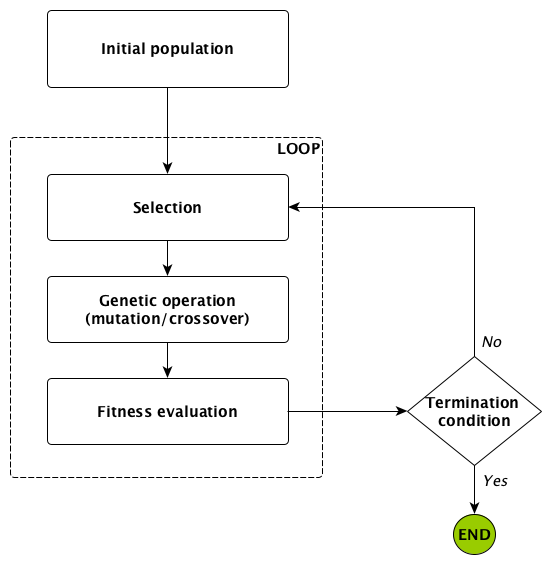
\includegraphics[width=1.4\linewidth]{../res/images/arnaque/EA_draw.png}
%	Evolutionary algorithm flow diagram}
\begin{itemize}
	\item Initialization: generating a random initial population of \ac{RNA} sequences compatible with the given target secondary structure.
	\item Evaluation and selection: evaluating a population of \ac{RNA} sequences consists of two steps: 1) fold each sequence into a secondary structure and assign it a weight based on its similarity to the target structure. 2) select a weighted random sample with replacement from the current population to generate a new population. A detailed description of the objective function used in our proposed tool \texttt{aRNAque} is provided in the next chapter. 
	\item Mutation (or move) operation: define a set of rules or steps used to produce new sequences from the selected or initial ones. This component is elaborated further in the next chapter.
	
\end{itemize}

\texttt{MODENA} uses a multi-objective function that measures the stability of the folded sequence and its similarities to the target. It starts from a population of randomly generated sequences, and the objective is optimized through tournament selection and random mutation at non-closing loop positions. 

In contrast, \(\texttt{ERD}\) starts by decomposing the target structure into loops and independently uses an evolutionary algorithm to minimize each constituent's energy. It was first developed in 2014 \cite{esmaili2014evolutionary}, and one year after, an updated version was released \cite{esmaili2015erd}. The main lines of \texttt{ERD} are:
\begin{enumerate}
	\item Pool reconstruction: using a collection of \ac{RNA} sequences (STRAN database) similar to the natural ones, a pool of sequences is constructed for their length by successively finding the corresponding structure using \texttt{RNAfold}, decomposing the structure in sub-components, and finally, the corresponding sub-sequences of the same size are gathered to form a pool. 
	\item Hierarchical decomposition of the target structure into loops: using the idea that any secondary structure can be uniquely decomposed into its structural components (stems, hairpin loops, internal loops, bulge and multi-loops), \texttt{ERD} decomposes the target in the positions where multi-loops occur. 
	\item Sequence initialization: after decomposing the target structure into sub-components,  for each sub-component, a random sub-sequence is chosen from the pool, and the initial sequence is a combination of those sub-sequences; 
	\item Evolutionary optimization of the sub-sequences: an EA algorithm is performed on each sub-component to improve the initial sequence. The outcome sub-sequences are combined to form a newer sequence that will replace the initial one.  Iteratively the evolutionary algorithm is performed on the updated sequence until the combined sequence folds into the target or in a failure case when the stopping condition is satisfied. Two evolutionary operators are implemented here, a mutation that consists of replacing a sub-sequence corresponding to a sub-component with a new random one from the pool for the same length, and a selection which consists of choosing from a population of $15$ \ac{RNA} sequences or sub-sequences, three best sequences with respect to their free energy and adding them to the best from the preview generation, three best ones with respect to the Hamming distance from the target are therefore chosen.  The next-generation population is then obtained by generating five new sequences for each of the three best sequences.
\end{enumerate}

In the different \ac{EA} methods presented above, the mutation operation is essential for good performance because it provides the rules that allow for navigating the solution space. \texttt{ERD} implements a non-local mutation, which consists of randomly changing a subsequence in the candidate solution with a new one taken from a set of possible moves. In contrast, \texttt{Modena} uses both local mutation and crossover operation to improve its search. However, both \acp{EA} present difficulties in finding RNA sequences that fold into some secondary structures of the \texttt{Eterna100} data set. That limitation could be due to the local search (for \texttt{Modena}) or the finite set of move data used in the non-local search implemented in \texttt{ERD}. In mathematical optimization, local searches are known for their quick convergence to a local minimum. This could be the same case for \acp{EA} implementing local mutations. To avoid early convergence \ac{EA} practitioners often implement non-local mutation methods, e.g. Lévy search, inspired by the Lévy flights. The following section describes the Lévy flight and reviews some applications of Lévy search in the context of \acp{EA}.

\subsubsection{Lévy flights and evolutionary algorithms}
In this section, we define concepts such as Lévy flights and provide a brief review of its implications and applications to optimization techniques such as evolutionary algorithms.

In its classical setting, evolutionary algorithms are guided by local (or one-point mutations) mutations. Although a local search can efficiently discover optima in a simple landscape, more complex landscapes pose challenges to designing evolutionary algorithms that rely solely on local search. This is especially true on a landscape with high neutrality where local search may be inefficient or risk getting stuck on a plateau (or local optimum). To avoid this pitfall, many practitioners suggested EA that implements a mutation scheme inspired by Lévy flights (called Lévy mutation).

Lévy flights are random walks with a Lévy (or any heavy-tailed) step size distribution. The concept originates in the work of Mandelbrot on the fluctuation of commodities prices in the 1960s \cite{mandelbrot1972certain} but has since found many more physical applications \cite{shlesinger1995levy}. The term "Lévy flight" was also coined by Mandelbrot, who used one specific distribution of step sizes (the Lévy distribution, named after the French mathematician Paul Lévy). Lévy flights also play a key role in animal foraging, perhaps because they provide an optimal balance between exploration and exploitation \cite{viswanathan2008levy,kamaruzaman2013levy}. For a recent review of applications of Lévy flights in biology from the molecular to the ecological scale, \cite{reynolds2018current}.

Similar to a Lévy flight, a Lévy mutation scheme allows simultaneous search at all scales over the landscape. New mutations most often produce nearby sequences (one-point mutations), but occasionally generate mutant sequences which are far away in genotype space (macro-mutations). In this work, the distribution of the number of point mutations at every step is taken to follow a Zipf distribution \cite{newman2005power}. 

Earlier works have applied similar ideas in genetic programming  \cite{LevyGP}, and in differential evolutionary algorithms \cite{sharma2015modified}. This motivated us to investigate a possible benefit of a Lévy flight in the design of \ac{RNA} sequences in \autoref{ch:arnaque}. In addition to \ac{EA} methods, there exists several computational RNA design tools implementing different techniques such as, \ac{ML}, \ac{NMCS} etc... The following section provides a short description of such tools.

\subsubsection{Tools implementing non-EA strategies.}

Several tools dealing with the \ac{RNA} folding problem implement different strategies from the population-based, or evolutionary algorithm approaches. This section describes couple of them, emphasising on those that are used in the benchmark results in \autoref{ch:arnaque}, which are \texttt{NEMO}, \texttt{RNAinverse}, \texttt{antaRNA} and\texttt{sentRNA}. 

\texttt{sentRNA} \cite{shi2018sentrna} is a computational agent that uses a set of information and strategies collected from the \texttt{EteRNA} game players to train a neural network model. The neural network assigns an identity of A, U, C, or G to each position in the given target, a featured representation of its local environment. The featured representation combines information about its bonding partner, nearest neighbours, and long-range features. While the bonding partner and nearest neighbour information are provided to the agent by default, long-range features are learned through the training data. For each target structure, the long-range features refer to the important position $j$ relative to $i$ that the agent should know about when deciding what nucleotide to assign to $i$. These are defined by two values: the Cartesian distance and the angle in radians. Those two values are computed for each position $(i,j)$ using a mutual information metric over the player solution dataset. Therefore, the result is a list of long-range features for a given target structure. A subset of long features is selected from this list and used to define a model for the neural network model's training, validation, and testing. In addition to the neural network model, \texttt{sentRNA} also implements a refinement algorithm on the unsuccessful design. The refinement algorithm is an adaptive walk that starts from the predicted sequence and uses a set of random mutations that allow improving the neural network solution. Alternatively, \texttt{EternaBrain} \cite{koodli2019eternabrain} implement a convolutional network model trained on a huge \texttt{EteRNA} moves-select repository of $30,477$ moves from the top $72$ players; and \texttt{LeaRNA} \cite{runge2018learning} uses deep reinforcement learning to train a policy network to sequentially design an entire \ac{RNA} sequence given a specified target structure.

\texttt{NEMO} \cite{nemo2018} is a recently developed tool combining a \ac{NMCS} technique with domain-specific knowledge to create a novel algorithm. The underlying idea is to start with an input pattern sequence of N's of the same length as the targeted structure. First, it uses the standard \acp{NMCS} to sample sequence solutions acting on N's only. A sequence candidate is selected from the sample; then folded into an \ac{MFE} structure. When the \ac{MFE} structure does not match the target, some subset mutations are performed, and a set of random mutated positions are picked to generate a new input pattern sequence. The new input pattern will allow sampling acting on N's only using the same standard \acp{NMCS}. This procedure is then repeated several times until the \ac{MFE} structure matches the targeted structure or not in the unsuccessful cases. The statistical results show that \texttt{NEMO} surpasses all the existing tools on the \texttt{EteRNA100} benchmark datasets by solving $\approx95\%$ of the targets using the Turner1999 energy parameter sets. Using a similar technique, \texttt{RNAinverse}\cite{lorenz2011viennarna}, one of the oldest inverse folding tools included in the \texttt{ViennaRNA} package, uses an adaptive random walk to minimize base-pair distance. The distance is computed by comparing the \ac{MFE} structure of the mutated sequence with the target structure. In addition, \texttt{RNAinverse} allows for designing more probable sequences using the partition function optimization. The latter allows for more stable designed sequences that mostly fold into \ac{MFE} structures different from the target structure. On an attempt to improve \texttt{RNAinverse}, many other tools have been suggested \texttt{INFO-RNA} \cite{busch2006info}, \texttt{RNA-SSD} \cite{andronescu2004new} and \texttt{DSS-Opt} \cite{matthies2012dynamics}. The most recent tools also include \texttt{RNAPOND} \cite{yao2021taming} and \texttt{MaiRNAiFold} \cite{minuesa2021moirnaifold}.

\(\texttt{antaRNA}\)~\cite{kleinkauf2015antarna} is also a recent program available since 2015, and it provides a web server for friendly usability. It utilizes an \textit{ant-colony} optimization, in which an initial sequence is generated via a weighted random search, and the \textit{fitness} of that sequence is then used to refine the weights and improve subsequences over generations. It provides many other interesting features, such as the sequence and target GC-content constraints. It also provides a fast python script that includes the options from the web server presented through a command line. Other tools also provide this dual advantage but implement different optimization techniques. \(\texttt{NUPACK:design}\) \cite{zadeh2011nucleic} uses a tree decomposition technique and the ensemble defect as objective function to design qualitatively good sequences. \texttt{incaRNAfbinv} \cite{drory2016incarnafbinv} is a program for fragment-based \ac{RNA} design. \texttt{incaRNAfbinv}'s web server combines two complementary methodologies: \(\texttt{IncaRNAtion}\) \cite{reinharz2013} and \texttt{RNAfbinv} \cite{weinbrand2013rnafbinv}. \(\texttt{IncaRNAtion}\) generates a GC-weighted partition function for the target structure, and then adaptively samples sequences from it to match the desired GC-content. \(\texttt{RNAiFold}\) \cite{garcia2013rnaifold} employs constraint programming that exhaustively searches over all possible sequences compatible with a given target. \(\texttt{RNAiFold}\) \cite{garcia2013rnaifold} has the particularity of  designing synthetic functional \ac{RNA} molecules.  

So far, except for \texttt{Modena} and \texttt{antaRNA}, most of the computation tools presented in previous sections do not account for pseudoknotted RNA target structures, which represents a disadvantage, knowing their implications in realizing \ac{ncRNA} biological functions. The following section reviews existing RNA design tools that support pseudoknotted secondary structures. 


\subsection{Pseudoknotted RNA inverse folding tools}
Designing \ac{RNA} sequences for pseudoknotted targets is computationally more expensive than pseudoknot-free targets. For that reason, many of the studies addressing the inverse folding of \ac{RNA} considered only pseudoknot-free secondary structures. There are, however, some exceptions: \texttt{MCTS-RNA} \cite{yang2017rna}, \texttt{antaRNA}\cite{kleinkauf2015antarna}, \texttt{Modena} and \texttt{Inv}\cite{gao2010inverse}. The computation tool presented in \autoref{ch:arnaque} of our work also considers pseudoknots. This section gives an overview of each of these tools. 

\texttt{Inv} was one of the first inverse folding tools handling pseudoknotted \ac{RNA} target structures, but it was restricted to a specific type of pseudoknot pattern called $3$-crossing nonplanar pseudoknots.

More recently, \texttt{MCTS-RNA}'s authors suggested a new technique that deals with a broader type of pseudoknots. It uses a \ac{MCTS} technique which has recently shown exceptional performance in Computer Go. The \ac{MCTS} allows initialising a set of \ac{RNA} sequence solutions in \texttt{MCTS-RNA} and the solutions are further improved through local updates at the nucleotide positions.

Another approaches (\texttt{Modena}, \texttt{antaRNA}) implements different strategies one which is a multi-objective \texttt{ant-colony} optimisation and the another one which is a multi-objective evolutionary algorithm.  Although the first versions were implemented for pseudoknot-free structure \cite{taneda2011modena, kleinkauf2015antarna}, they have since been extended to support pseudoknotted \acp{RNA} \cite{modena_2012, kleinkauf2015antarna2}. 

Each of the tools mentioned above rely on a folding tools that predicts pseudoknotted secondary structure: \texttt{MCTS-RNA} uses \texttt{pkiss} whereas the other tools (\texttt{antaRNA} and \texttt{Modena}) support two folding tools such as \texttt{HotKnots} and \texttt{IPKnot}. In the context of this work, two folding tools are used \texttt{HotKnots} and \texttt{IPKnot}, and they support the two main types of pseudoknot patterns (i.e. H-type and K-type) contained in the benchmark data used to evaluate our result in \autoref{ch:arnaque}. Both pseudoknotted and pseudoknot-free benchmark data sets are considered in this work. The following section describes the benchmark data used to evaluate our proposed \ac{EA} tool.

\section{Benchmarking the Inverse folding tools}
\label{sec:benchmark_data}
The validation of the designed \ac{RNA} sequences using computational methods often requires biological experiments. Because of the high cost of experimental techniques, most investigators limit their guarantee to using benchmark datasets \cite{churkin2017design} in general. For pseudoknot-free design tools,  two benchmark datasets are mostly used in the literature---$(i)$ \texttt{RFAM} \footnote{The Rfam database \url{https://rfam.xfam.org/}}: a collection of \ac{RNA} families, each represented by multiple sequence alignments, consensus secondary structures and covariance models---$(ii)$ \texttt{Eterna100} \cite{anderson2016principles}: a collection of hundred \ac{RNA} secondary structures extracted from the EteRNA Puzzle game\footnote{The EteRNA game \url{https://eternagame.org/}}. For \ac{RNA} inverse tools that support pseudoknots, the \texttt{PseudoBase++}\cite{taufer2009pseudobase++} dataset is often considered. This section provides references, descriptions and the cleanup procedure applied for the three data sets mentioned above.


The \(\texttt{Eterna100}\) dataset \cite{Eterna} is available in two versions and both contain a set of \(100\) target structures extracted from the \texttt{EteRNA} puzzle game and classified by their degree of difficulty. The \texttt{Eterna100-V1} was initially designed using \texttt{ViennaRNA} 1.8.5, which relies on Turner1999 energy parameters \cite{Turn1999}. Out of the $100$ target secondary structures, $19$ turned out to be unsolvable using the version of \texttt{ViennaRNA} $2.4.14$ (which relays on the Turner2004 \cite{mathews2004incorporating}). Subsequently, an \texttt{Eterna100-V2} \cite{Eterna} was released in which the $19$ targets were slightly modified to be solvable using \texttt{ViennaRNA} $2.4.14$ and any version that supports the Turner2004 energy parameters. The main difference between the two dataset relay on the energy parameters used to generate the data.

The \texttt{non-EteRNA} (a subset of the \texttt{RFAM}) dataset in a set of \(63\) experimentally synthesized targets that Garcia-Martin et al. \cite{garcia2013rnaifold} recently used to benchmark a set of ten inverse folding algorithms, which from our knowledge, is the most recent and comprehensive benchmark of current state-of-the-art methods. The dataset is collected from \(3\) sources: the first dataset called \(\textbf{dataset A}\) which contains \(29\) targets collected from RFAM and also used in \cite{esmaili2015erd,taneda2011modena} and the second called \(\textbf{dataset B}\) is a collection of \(24\) targets used in \cite{esmaili2015erd} and added to that the \(10\) structures used in \cite{shi2018sentrna}.

The \texttt{PseudoBase++} is a set of $266$ pseudoknotted \ac{RNA} structures used to benchmark \texttt{Modena}. It was initially $342$ \ac{RNA} secondary structures, but because of the redundancy and the non-canonical base-pairs  $76$ structures were excluded. To group the dataset with respect to the pseudoknot motifs, we used the test data from \texttt{antaRNA}'s paper. The test data contains $249$ grouped into four categories: $209$ hairpin pseudoknots (H), $29$ bulge pseudoknots (B), $8$ complex hairpin pseudoknots (cH) and $3$ kissing hairpin pseudoknots (K). Out of the $266$ structures, only $185$ (with $150$ H-type, $3$ K-type, $25$ B-type and $7$ cH-type) structures were included in the test data. So for that reason, we have used only $185$ target structures for the pseudoknot motif performance comparison and the $266$ structures for the different target lengths performance comparison.

When the benchmark datasets rely on a particular energy parameter set, the performance of a given inverse \ac{RNA} folding tool evaluated on these datasets will also be related to the choice of the \ac{RNA} folding tool's energy parameter set. If the benchmark datasets do not rely on a particular energy parameter set, the robustness of the inverse \ac{RNA} tool will be its capability to perform well on different energy parameter sets.

\section{Conclusion}
In summary, the \ac{RNA} inverse folding problem is still computationally challenging because there are many objective functions and different ways of evaluating computational tools. Solving this problem is particularly interesting in \ac{RNA} synthetics, \ac{RNA} nanostructure design, and emerging fields such as bioengineering. We presented a comprehensive literature review of existing computational methods that addressed this problem in this chapter. The existing approaches have some advantages and disadvantages, depending on the techniques implemented. \(\texttt{NUPACK}\) for example---despite its well-defined objective function---still has difficulty designing sequences for large targets and most of the \(\texttt{EteRNA100}\) targets. In contrast, \(\texttt{ERD}\) because of its powerful decomposition method, which allows dealing quickly with large targets (On \text{RFAM} 1.0 with target's length between~\(400-1400\)) but is still a big challenge to solve more than~\(65\%\)~of the~\(\texttt{EteRNA100-V2}\) using the Turner2004 energy parameter sets. On another side,~\(\texttt{NEMO}\), one of the most recent tools, can solve more than~\(90\%\)~of~ the \(\texttt{EteRNA100-V1}\) dataset using an old version of \texttt{ViennaRNA} package, which is based on Turner1999 energy parameter sets~\cite{Turn1999}. The \texttt{sentRNA}'s machine learning model also relied on the same old version of \texttt{ViennaRNA} package and, by adding a refinement on the machine learning model, \texttt{sentRNA} solves~\(78\%\)~of~\(\texttt{EteRNA100}\). Without this refinement,~\(\texttt{sentRNA}\) can only solve \(48\%\) of \(\texttt{EteRNA100}\)'s targets, which can represents another limitation. For the EAs \texttt{ERD} and \texttt{MODENA}, none of them can solve more than~\(65\%\)~of~\(\texttt{EteRNA100}\) using the Turner2004 energy parameter sets.  

In the next chapter, we will introduce a simple evolutionary algorithm called \texttt{aRNAque} that implements a Lévy mutation and allows significant improvements to the existing tools.
%*****************************************
%*****************************************
%*****************************************
%*****************************************
%*****************************************
